\documentclass[12pt]{article}
\usepackage[margin=2.5cm]{geometry}
\usepackage{enumerate}
\usepackage{amsfonts}
\usepackage{amsmath}
\usepackage{fancyhdr}
\usepackage{amsmath}
\usepackage{amssymb}
\usepackage{amsthm}
\usepackage{mdframed}
\usepackage{graphicx}
\usepackage{subcaption}
\usepackage{adjustbox}
\usepackage{listings}
\usepackage{xcolor}
\usepackage{booktabs}
\usepackage[utf]{kotex}
\usepackage{hyperref}
\usepackage{accents}

\definecolor{codegreen}{rgb}{0,0.6,0}
\definecolor{codegray}{rgb}{0.5,0.5,0.5}
\definecolor{codepurple}{rgb}{0.58,0,0.82}
\definecolor{backcolour}{rgb}{0.95,0.95,0.92}

\lstdefinestyle{mystyle}{
    backgroundcolor=\color{backcolour},
    commentstyle=\color{codegreen},
    keywordstyle=\color{magenta},
    numberstyle=\tiny\color{codegray},
    stringstyle=\color{codepurple},
    basicstyle=\ttfamily\footnotesize,
    breakatwhitespace=false,
    breaklines=true,
    captionpos=b,
    keepspaces=true,
    numbers=left,
    numbersep=5pt,
    showspaces=false,
    showstringspaces=false,
    showtabs=false,
    tabsize=1
}

\lstset{style=mystyle}

\pagestyle{fancy}
\renewcommand{\headrulewidth}{0.4pt}
\lhead{CSC 343}
\rhead{Worksheet 10}

\begin{document}
\title{CSC343 Worksheet 10}
\maketitle

\bigskip

\begin{enumerate}[1.]
    \item \textbf{Exercise 12.1.1:} Figures 12.4 and 12.5 are the beginning and end, respectively,
    of an XML document that contains some of the data from our running
    products exercise. Write the following XPath queries. What is the result of
    each?

    \begin{center}
    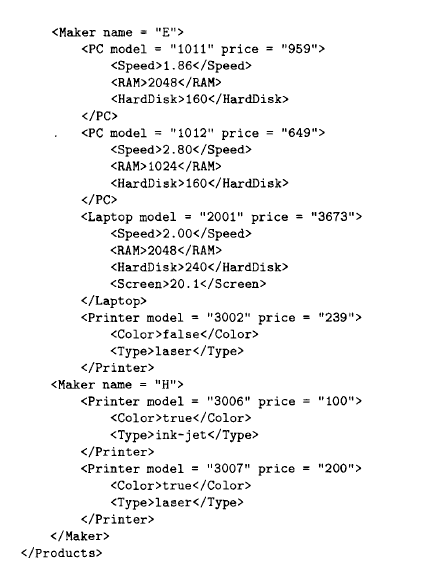
\includegraphics[width=0.7\linewidth]{images/worksheet_10_1.png}
    \end{center}

    \bigskip

    \begin{enumerate}[a)]
        \item Find the amount of RAM on each PC.
        \item Find the price of each product of any kind.
        \item Find all the printer elements.
        \item Find the makers of laser printers.
        \item Find the makers of PC's and/or laptops.
        \item Find the model numbers of PC's with a hard disk of at least 200 gigabytes.
    \end{enumerate}

    \item \textbf{Exercise 12.1.2:} The document of Fig. 12.6 contains data similar to that
    used in our running battleships exercise. In this document, data about ships is
    nested within their class element, and information about battles appears inside
    each ship element. Write the following queries in XPath. What is the result of
    each?

    \begin{center}
    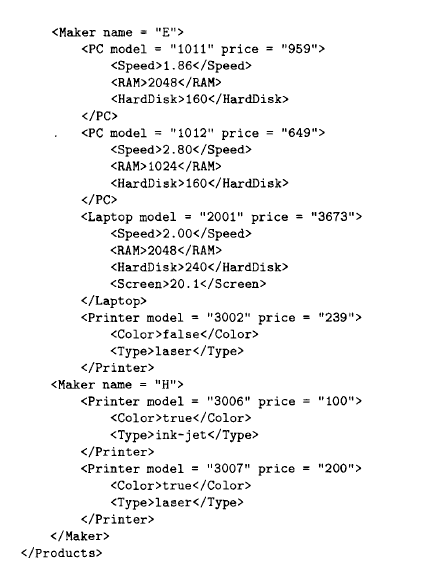
\includegraphics[width=0.7\linewidth]{images/worksheet_10_1.png}
    \end{center}

    \bigskip

    \begin{enumerate}[a)]
        \item Find the names of all ships.
        \item Find all the Class elements for classes with a displacement larger than 35000.
        \item Find all the Ship elements for ships that were launched before 1917.
        \item Find the names of the ships that were sunk.
        \item Find the years in which ships having the same name as their class were launched.
        \item Find the names of all ships that were in battles.
    \end{enumerate}

    \item \textbf{Exercise 12.2.1:} Using the product data from Figs. 12.4 and 12.5, write the
    following in XQuery.

    \bigskip

    \begin{enumerate}[a)]
        \item Find the Printer elements with a price less than 100.
        \item Find the Printer elements with a price less than 100, and produce the sequence of these elements surrounded by a tag $<$CheapPrinters$>$.
        \item Find the names of the makers of both printers and laptops.
        \item Find the names of the makers that produce at least two PC's with a speed of 3.00 or more.
        \item Find the makers such that every PC they produce has a price no more than 1000.
    \end{enumerate}

    \item \textbf{Exercise 12.2.2:} Using the battleships data of Fig. 12.6, write the following
    in XQuery.

    \bigskip

    \begin{enumerate}[a)]
        \item Find the names of the classes that had at least 10 guns.
        \item Find the names of the ships that had at least 10 guns.
        \item Find the names of the ships that were sunk.
        \item Find the names of the classes with at least 3 ships.
        \item Find the names of the classes such that no ship of that class was in a
    \end{enumerate}


    \item \textbf{Exercise 12.2.3:} Solve the problem of Section 12.2.5; write a query that finds
    the star(s) living at a given address, even if they have several addresses, without
    finding stars that do not live at that address.

    \item \textbf{Exercise 12.2.4:} Do there exist expressions $E$ and $F$ such that the expression
    every \$x in $E$ satisfies F is true, but some \$x in $E$ satisfies $F$
    is false? Either give an example or explain why it is impossible.
\end{enumerate}

\end{document}